\documentclass[border=2pt]{standalone}
\usepackage{tikz}
\usetikzlibrary{arrows.meta}

\definecolor{orangeText}{HTML}{E3A063}
\definecolor{orangeDim}{HTML}{A87A4E}
\begin{document}
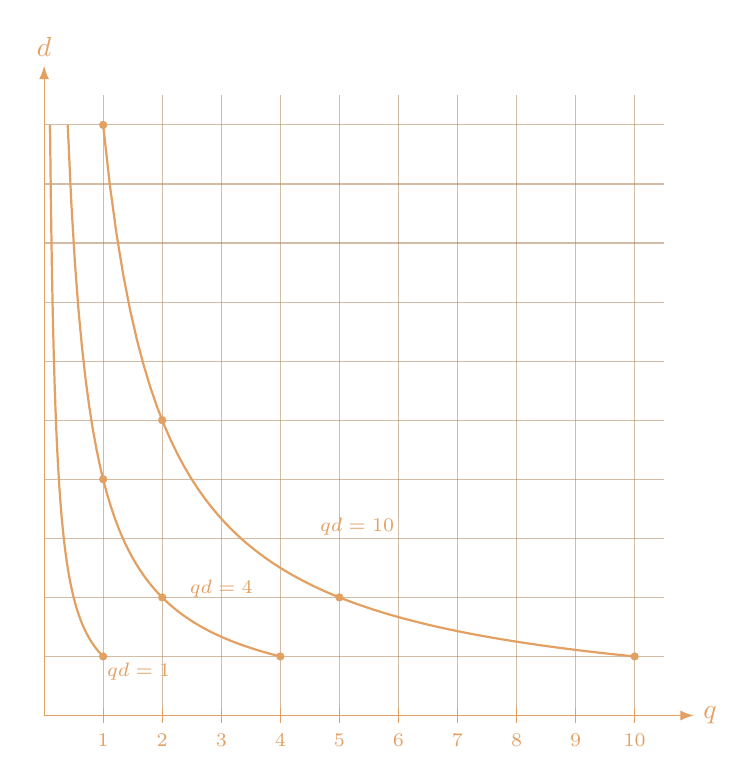
\begin{tikzpicture}[color=orangeText, >=Latex, scale=0.75]

    % grid
    \foreach \i in {1,...,10} {
        \draw[orangeDim, opacity=0.5] (\i,0) -- (\i,10.5);
        \draw[orangeDim, opacity=0.5] (0,\i) -- (10.5,\i);
    }

    % axes
    \draw[->] (0,0) -- (11,0) node[right] {$q$};
    \draw[->] (0,0) -- (0,11) node[above] {$d$};

    % hyperbolas qd = k
    \draw[thick] plot[domain=0.1:1,samples=60] (\x,{1/\x});
    \draw[thick] plot[domain=0.4:4,samples=60] (\x,{4/\x});
    \draw[thick] plot[domain=1:10,samples=80] (\x,{10/\x});

    \node at (1.6,0.75) {\scriptsize $qd=1$};
    \node at (3.0,2.15) {\scriptsize $qd=4$};
    \node at (5.3,3.2) {\scriptsize $qd=10$};

    % lattice points on qd = 1
    \fill (1,1) circle (2pt);

    % lattice points on qd = 4
    \fill (1,4) circle (2pt);
    \fill (2,2) circle (2pt);
    \fill (4,1) circle (2pt);

    % lattice points on qd = 10
    \fill (1,10) circle (2pt);
    \fill (2,5) circle (2pt);
    \fill (5,2) circle (2pt);
    \fill (10,1) circle (2pt);

    \foreach \i in {1,...,10} {
        \draw (\i,-0.12) -- (\i,0.12);
        \node[below] at (\i,-0.15) {\scriptsize \i};
    }

\end{tikzpicture}
\end{document}
